%%%%%%%%%%%%%%%%%%%%%%%%%%%%%%%%%%%%%%%%%%%%%%%%%%%%%%%%%
%%%%%%%%%%%%%%%%% author:dormir_yin %%%%%%%%%%%%%%%%%%%%%%%%%%%%%%
%%%%%%%%%%%%%%%%%%%%%%%%%%%%%%%%%%%%%%%%%%%%%%%%%%%%%%%%%

\chapter{序列模型:循环网络与递归网络}
\label{chap:10}
循环神经网络(Recurrent neural networks,简称RNN),是一系列处理序列数据(sequential data)的神经网络的统称。前面的章节我们介绍的卷积神经网络是专门来处理格状结构的数据X的,比如说图像。而循环神经网络是用来处理序列的,序列一般表示为:$x^{(1)}...x^{(\tau)}$\footnote{译者注:序列数据可以是时间序列,可以是空间序列,当然也可以是其他形式的的序列。为了便于理解我们假设我们处理的是时间序列,上标对应的是不同的时间点。每个时间点对应的输入向量是$x^{(t)}$}。我们已经知道卷积神经网络在处理长宽都很大的图像和处理小图像模型并没有很大的不同,甚至有的卷积神经网络模型可以处理大小不固定的输入图像。递归神经网络也有类似能力,当递归神经网络处理序列时,并不需要针对不同长度的序列分别设计一个模型。大部分递归神经网络模型可以处理长度变化的输入序列。

在我们介绍循环神经网络之前,首先向大家介绍一下在八十年代机器学习和统计模型领域提出的一个观点:在模型的不同部分共享参数(sharing parameters)。参数共享可以帮助我们扩展模型,让模型去处理不同形式(在这里主要是不同长度的序列)的输入数据。处理序列数据时,如果我们对序列中每个不同的时间点对应的输入元素使用不同的参数,我们就不能处理长度未知的序列,训练的过程中也不能享有统计优势(statistical strength)\footnote{译者注;感觉作者想要表达的意思是序列中每个元素有可能都不是相互独立的,我们如果使用参数共享,可以从整体来提取一些共性的东西。举个例子,如果数据集是从某个分布采样得到的,如果我们对这个数据的整体来处理,反而更容易得到这个分布的信息}。当某个有用的信息在序列的不同位置都有可能出现时,参数共享就变得尤为重要。举个例子:比较两个句子“I went to Nepal in 2009”  和 “In 2009,I went to Nepal.”,如果我们把这两个句子输入机器学习模型,让模型把叙述者去Nepal的年份给提取出来,我们期望模型识别2009作为有用的信息,尽管这个词在这个两个句子中出现的位置不一样:一个是第六个单词,一个是第二个单词。假设我们用前馈神经网络处理句子。一个传统的全连接前馈神经网络只能处理固定长度的句子序列,对序列不同位置或者不同时间点的输入的特征都对应不同的参数,所以它需要学习句子中每个位置所对应的语法规则。与传统的全连接网络不同,循环神经网络在序列的每个时间点所对应的权值参数是一样的,也就是说序列不同位置的输入特征会共享参数。

其实当我们在在1维时间序列(1-D temporal sequence)中使用卷积的时候,也使用了参数共享。序列1维卷积的方法也是时间延迟神经网络(time-delay neural networks)的基础(Lang and Hinton, 1988; Waibel et al., 1989; Lang et al., 1990)。卷积操作允许神经网络在不同的时间上共享权值。但是这个网络特别浅。序列经过卷积之后,它的输出依然是一个序列。输出序列的每个成员是对应位置输入与周围相邻的输入经过某个函数的映射输出。在每个时间点我们都使用了相同的卷积核,这也正体现了前面所提的参数共享的观点。在循环神经网络中,参数共享是以另一种方式实现的。1维卷积只考虑对应位置附近的特征,而在RNN中每个输出序列里的成员都是之前所有的输出经过一个函数映射得到的。也就是说在产生当前时间点输出的时候,我们要考虑之前所有的输出。在计算输出序列每个成员的时候会考虑所有的历史输出,而所采取的映射规则是一致的。如果用计算图来展示这个递归模式,会发现是在一个非常深的计算图中做参数共享。

为了便于理解,我们记RNN处理的序列数据为一系列向量$\bm{x}^{(t)}$。$t$表示向量在序列中的位置,我们可以理解为时间点,范围是从$1$到$\tau$。在实际应用中,RNN通常分批次(minibatch)处理序列,每个minibatch里序列的长度$\tau$可能不一样。为了简化,我们没有在下标中标注批次。实际上,序列中向量的下标不一定要与现实生活中的时间对应起来,有的时候它仅仅表示该成员在序列中的位置。RNN有时也可以处理二维空间数据,比如说图像。在处理与时间有关的序列时,RNN还可以反向处理数据,或者说神经网络在处理序列之前已经将整个序列看了一遍。\footnote{这段现在解释起来有点难度,在看到双向循环神经网络就会理解了。} 

这章会对我们之前学过的计算图进行扩展,我们会看到带有环状结构的计算图。这个环表示当前时间点会作为一个变量影响未来时间点的值。这类计算图可以帮助我们定义循环神经网络。我们随后会展示用不同的方式构建,训练和使用循环神经网络。

如果你想了解更多和循环神经网络有关的内容,可以看一下Graves (2012)。

\section{计算图的展开}
\label{sec:10.1}
计算图可以形象的展示一系列计算操作,在神经网络中计算题可以清晰的展示如何将输入和模型参数映射成为输出和损失。可以从\ref{sec:6.5.1} 看一下更详细的介绍。在这一节我们将会解释如何将递归或者循环计算展开成具有重复结构的计算图,这个展开的计算题是一个链式结构。在展开过程中我们或看到如何在一个深的网络结构中使用参数共享。
举个例子,考虑一下典型的动态系统:
\begin{equation}
\bm{s}^{(t)} = f(\bm{s}^{(t-1)};\theta)
\label{form:10.1}
\end{equation}

其中$\bm{s}^{(t)}$表示当前系统状态。
等式\ref{form:10.1}是递归的因为$t$时刻状态$\bm{s}^{(t)}$的定义会使用到$t-1$时刻的状态$\bm{s}^{(t-1)}$定义,状态定义的方式是一样的,所以这个式子是递归的。

对于一个有限长的序列,假设他的长度是$\tau$,我们只需要重复使用$\tau-1$次上面的式子就可以把计算图展开。比如说我们要展开式子$\tau =3$,我们可以得到
\begin{eqnarray}
\bm{s}^{(3)} & = & f(\bm{s}^{(2)};\theta) \\
& = & f(f(\bm{s}^{(1)};\theta);\theta)
\end{eqnarray}
通过重复的调用等式\ref{form:10.1}来展开这个等式,我们可以得到一个不包含递归部分的表达式。这个表达式就可以用传统无环计算图来表示。式子\ref{form:10.1}对应展开的计算图可以看 
图\ref{fig:10_1}。
\begin{figure}[htbp] %  figure placement: here, top, bottom, or page
   \centering
   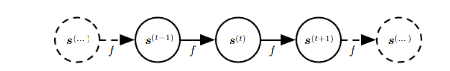
\includegraphics[width=6in]{fig/chap10/10_1.PNG} 
   \caption{这是一个展开的计算图,描述的是等式 定义的一个动态系统。每个节点代表不同时刻$t$的状态,函数$f$将$t$时刻的状态映射到$t+1$时刻的状态,每个$f$所使用的参数是一样的。}
   \label{fig:10_1}
\end{figure}

我们现在看另一个例子,我们考虑另一个动态系统,这个系统每次会接收一个外部的信号$\bm{x}^{(t)}$,
\begin{equation}
\bm{s}^{(t)} = f(\bm{s}^{(t-1)},\bm{x}^{(t)};\theta)
\label{form:10.4}
\end{equation}
我们可以看到当前状态包含所有之前时间点的历史信息。

循环神经网络可以用不同的方式来构建。我们所使用的函数几乎都可以看作是前馈神经网络(输入经过函数映射到输出),如果在函数外面再引入循环结构,那么就可以被看作循环神经网络。

很多神经网络用等式\ref{form:10.5} 或者类似式子来定义它们隐藏单元的值。为了这个状态是神经网络的隐藏单元,我们对式子\ref{form:10.4}进行了修改,用变量$h$来表示这个状态:
\begin{equation}
\bm{h}^{(t)} = f(\bm{h}^{(t-1)},\bm{x}^{(t)};\theta)
\label{form:10.5}
\end{equation}
这个式子对应的图是\ref{fig:10_2}典型的RNN会增加一个额外的结构,比如说输出层,从隐藏状态$h$中提取信息来作出预测。
\begin{figure}[htbp] %  figure placement: here, top, bottom, or page
   \centering
   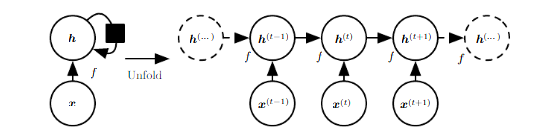
\includegraphics[width=6in]{fig/chap10/10_2.PNG} 
   \caption{一个没有输出的循环神经网络结构。网络会从输入$x$中提取信息,然后整合到隐藏状态$h$中,$h$会被传递下去作为下一个时间点输入的一部分。(左边)未展开的带环计算图。黑色的方块表示一个单位时间的延迟。(右边) 展开的计算图,本质和右边带环的图是一样的,每个节点对应一个特定的时间点。}
   \label{fig:10_2}
\end{figure}

等式\ref{form:10.5}可以用两种不同的方式来理解,我们用计算图来来帮助我们理解这两种思路。第一种可以看作是未展开的计算图,只包含有一个节点,我们甚至可以在现实中用物理实现这个模型。参考生物意义上的神经网络。在这个情况下,图中包含有一个环,它会实时的对网络进行操作。就像图\ref{fig:10_2} 左边的那个图一样。在本章中,我们在环中加了一个黑色的小方块来表示某个交互操作延后了一个时间单位,从$t$时刻的状态延后到$t+1$\footnote{译者注;这个地方不太好翻译,大家对照着图\ref{fig:10_2}去理解。}。另一种是用一个展开的计算图来描述RNN。图中有很多的节点,每个节点表示一个变量,这样每个时间点都对应一个变量来表示在那个时间点的状态。就像图\ref{fig:10_2}右边的那样。展开就是把图\ref{fig:10_2}左边带环的图映射到右边有重复结构的计算图的形式。展开的图的大小取决于序列的长度。

我们可以用函数$g^{(t)}$来表示经过$t$步展开之后的式子:
\begin{eqnarray}
\bm{h}^{(t)} & = & g^{(t)}(\bm{x}^{(t)},\bm{x}^{(t-1)},...,\bm{x}^{(2)},\bm{x}^{(1)}) \\
& = & f(\bm{h}^{(t-1)},\bm{x}^{(t)};\theta)
\end{eqnarray}

函数$g^{(t)}$把整个历史序列$(\bm{x}^{(t)},\bm{x}^{(t-1)},...,\bm{x}^{(2)},\bm{x}^{(1)})$都作为输入,输出为当前状态。但是展开的循环结构允许我们将函数用$f$来展开,我们只要递归调用函数$f$就可以得到函数$bm{h}$。展开过程有两个主要的优势:
\begin{enumerate}
\item 无论序列有多长,模型的输入变量的维度是一致的,因为从一个状态转到另一个状态的映射是固定的。而不是说把一个个长度不定的历史序列映射到一个个状态。
\item 我们每一步都可以使用一样的转换函数$f$,函数$f$的参数也可以共享。
\end{enumerate}

正因为这两个优势,我们可以只训练一个模型$f$, 这样我们不需要考虑序列的长度,每一步我们使用相同的$f$,不需要对所有可能的时间点都学习一个模型$g^{(t)}$。使用一个可以共享参数的模型能够允许我们将模型泛化到任意长度的序列中,即使某个序列的长度没有在训练集中出现。相比较不使用参数共享的模型,我们的模型在训练的时候只需要少量的训练数据。

循环图和展开图有不同的用处。循环图是简洁的。展开的计算图可以向我们展示每一步的计算,也可以展示信息流动的路径:如何沿着时间方向流动的(计算输出和损失),如何反着流动(计算梯度)。

\section{循环神经网络}
\label{sec:10.2}
在\ref{sec:10.1}我们介绍了计算图的展开和参数共享的思想。现在我们可以设计其他更复杂的递归神经网络模型。
\begin{figure}[htbp] %  figure placement: here, top, bottom, or page
   \centering
   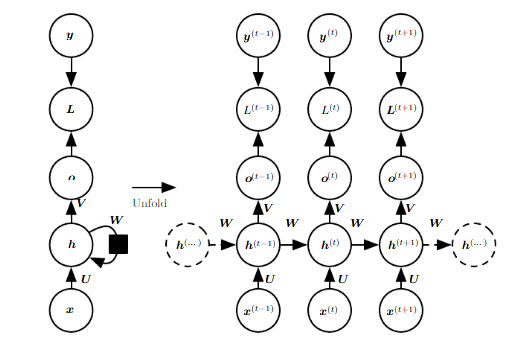
\includegraphics[width=6in]{fig/chap10/10_3.PNG} 
   \caption{这个计算图是用来展示如何计算循环神经网络训练过程中损失函数的值。这个循环神经网络会将输入序列$\bm{x}$映射到一个输出序列$\bm{o}$。损失函数$L$会在训练过程计算预测序列和对应的真实序列之间的距离。当我们使用softmax作为输出,我们假设$\bm{o}$是未归一化的对数概率。损失函数会首先计算$\hat{y}=softmax(\bm{o})$,然后将它和真实值$\bm{y}$进行比较。RNN使用权重矩阵$U$构建的映射关系,将输入映射到隐藏状态,隐藏状态到隐藏状态的映射是权重矩阵$W$来构建的,隐藏状态到输出状态的映射是有权重矩阵$V$来构建的。等式\ref{form:10.8}定义了这个模型的前向传播表达式。(左边)RNN模型和损失函数计算。(右边)将左边的计算图展开了,每个节点对应着一个特定的时间节点。}
   \label{fig:10_3}
\end{figure}

\begin{figure}[htbp] %  figure placement: here, top, bottom, or page
   \centering
   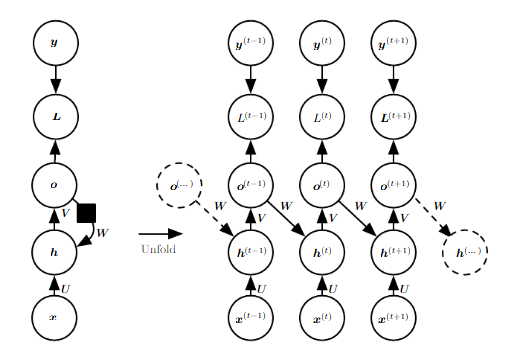
\includegraphics[width=6in]{fig/chap10/10_4.PNG} 
   \caption{在这个递归神经网络模型中,递归部分是输出指向下个时间点对应的隐藏状态的反馈。在每个时间点$t$, 输入是$\Vx_t$,隐藏层的节点是$\Vh^{(t)}$,输出是$\Vo^{(t)}$,真实值是$\Vy^{(t)}$,损失是$L^{(t)}$。(左边)带环的计算图。(右边)展开的计算图。这个模型和图\ref{fig:10_3}表示的RNN模型相比有一些局限(只能模拟很少的一部分函数),图\ref{fig:10_3}代表的模型可以将任意的历史信息存储到隐藏状态$\Vh$中,让后将$\Vh$传给之后的隐藏状态。这个图中的RNN需要把一个特制的输出值放进$\Vo$中,只有$\Vo$会被传递给之后的节点。无法直接从$\Vh$传递信息给后面的节点。之前的隐藏节点$\Vh$不能直接和当前的隐藏节点相连,只能通过它产生的输出来连接下一个隐藏节点。除非$\Vo$是一个维度非常大的向量,可以存储很多的信息,否则$\Vo$或丢失掉很多重要的历史信息。这就造成了这个模型有一些局限,但是这个模型很容易训练,因为每一步可以独立的进行训练,所以在训练过程中我们可以使用并行计算,这个我们在\ref{sec:10.2.1}中进行了介绍。}
   \label{fig:10_4}
\end{figure}

下面我们介绍了典型循环神经网络一些重要设计模式的例子:
\begin{itemize}
\item 循环神经网络每一时间点产生一个输出,隐藏单元之间互相联系,如图\ref{fig:10_3}。
\item 循环神经网络每一时间点产生一个输出,隐藏单元之和前一个时间点的输出有联系,如图\ref{fig:10_4}。
\item 循环神经网络的隐藏单元互相联系,在处理完整个序列之后常数一个输出,如图\ref{fig:10_5}。

\end{itemize}
本章主要介绍图\ref{fig:10_3}展示的模型。

图\ref{fig:10_3}和\ref{form:10.8}展示的循环神经网络模型是图灵完备的,任何可以被图灵机计算的函数也能够被一个有限大小的循环神经网络来计算。在一些时间步之后,计算RNN的输出的算法复杂度与和图灵机用的时间步的长度是线性渐进关系,和输入的长度也是线性渐进关系(Siegelmann and Sontag, 1991; Siegelmann, 1995; Siegelmann and Sontag, 1995;Hyotyniemi, 1996)。图灵机能计算的函数是离散的,所以这些结果注重精确的实现函数,而不是近似。当我们把RNN作为一个图灵机使用,输入为二进制序列,输出必须先离散化来使输出变成二进制。用一个单独特制有限大小的RNN在这个设置下计算所有可以模拟图灵机的函数是可行的(Siegelmann andSontag (1995) use 886 units)。图灵机的输入是一个特制的需要计算函数,所以一个能够模拟图灵机的RNN可以解决所有问题。理论上的RNN可以模拟无线堆栈,只要将他的激活值和权重由无限精度的有理数来表示。\footnote{这段感觉主要讲RNN是图灵完备的,那几篇论文主要证明了RNN和图灵机的等价。如果没学过计算复杂性理论我觉得没必要看了。后面讲了无限堆栈,不知道和数据结构里的堆栈有啥联系,不是很懂。大家这段可以略过,不影响之后的内容。}

我们现在已经得到了图\ref{fig:10_3}描述的RNN前向传播的公式。但是这个图并没有表明隐藏单元使用的激活函数。这里我们假设他使用的激活函数是是双曲正切(tanh)。这个图也没有展示输出和损失函数的形式。这儿我们假设输出是离散的,因为RNN经常被用来预测单词和字母。一个很自然表示离散变量的方式是把输出$\Vo$看作是一个对于离散变量,每个可能的值赋予一个未被归一化的对数概率。然后我们就可以通过softmax操作作为来处理刚刚的数据,这样就可以得到归一化之后的输出概率$\hat \Vy$。前向传播从初始值$\Vh^{(0)}$开始。然后接下来每一步,从$t= 1$到$t = \tau$我们使用下面的公式递归来完成:
\begin{align}
\label{eq:108a}
 \Va^{(t)} &= \Vb + \MW \Vh^{(t-1)} + \MU \Vx^{(t)}, \\
  \Vh^{(t)} &= \tanh(\Va^{(t)} ), \\
  \Vo^{(t)} &= \Vc + \MV \Vh^{(t)}, \\
  \hat \Vy^{(t)} &= \text{softmax}(\Vo^{(t)}),
\end{align}
这些公式里面的参数有偏置向量$\Vb$和$\Vc$,以及权重矩阵$\MU$、$\MV$和$\MW$,这些权重矩阵分别对应三个函数映射。输入到隐藏状态,隐藏到输出状态,隐藏到隐藏状态。这个例子展示了循环神经网络如何将输入序列映射到相同长度的输出序列。计算损失时我们得根据输入序列$\Vx$,和对应的目标序列$\Vy$,然后我们把每个时间点对应的损失都加起来。比如说,如果损失$L^{(t)}$我们选给定 $\Vx^{(1)}, \dots, \Vx^{(t)}$情况下$\Vy^{(t)}$的下负对数似然(negativelog-likelihood),那么:
\begin{align} \label{eq:1012L}
 & L\big( \{ \Vx^{(1)}, \dots, \Vx^{(\tau)} \}, \{ \Vy^{(1)}, \dots, \Vy^{(\tau)}  \} \big) \\
 & = \sum_t L^{(t)} \\
 & = - \sum_t \log p_{\text{model}} \big(  y^{(t)} |  \{ \Vx^{(1)}, \dots, \Vx^{(t)} \} \big) ,
\end{align}
其中$p_{\text{model}} \big(  y^{(t)} |  \{ \Vx^{(1)}, \dots, \Vx^{(t)} \} \big) $是需要我们计算模型的输出$\hat \Vy^{(t)}$中对应目标值$y^{(t)}$的信息\footnote{译者注: 此处不确定,感觉原文有误,entry应该为entropy,希望在之后的校对中解决这个问题}。计算参数在该损失函数中的梯度计算很复杂。计算梯度的时候我们需要先从左到右使用前向传播算法,正如展开图\ref{fig:10_3}一样,接着从右到左使用后向传播算法。时间复杂度是$\CalO(\tau)$, 而且这个过程不能通过并行计算来提速。因为前向计算时是有顺序的。必须要先计算好一个然后再计算下一个。前向计算的所有结果必须先储存起来,因为在后向计算的时候会被用到,后向计算用完之后就可以销毁了。所以算法的存储复杂度也是$\CalO(\tau)$,当我们把后向传播算法应用搭配RNN的展开图中的时候,复杂度为$\CalO(\tau)$,我们叫这个算法的名字是随着时间后向传播算法(back-propagation through time)简称 BPTT。这个算法的细节会在\ref{sec:10.2.2}讲。这个在隐藏状态之间存在递归的网络是非常强大的,但是训练需要很多时间。有没有可以替代的方案呢?

\subsection{老师驱动(Teacher Forcing)以及有循环输出的神经网络}
\label{sec:10.2.1}
如果神经网络的递归部分存在于每一步的输出和下一步的隐藏单元的连接中,网络的能力会比较小。因为它缺少隐藏状态之间的递归联系。举个例子,它不能模拟一个通用图灵机。由于网络结构缺少隐藏层之间的联系,它需要输出单元能够将所有的历史信息都保存起来,然后网络可以用来预测未来信息。因为输出单元主要是用来匹配训练集的目标的,而不是用来从历史输入中提取有用的信息。除非使用者已经知道如何描述系统的所有状态,然后把他作为训练集目标输出的一部分,这个时候存储有用信息和输出尽量与目标相等这两个任务就重合了。把隐藏单元到隐藏单元的递归关系去掉的好处是: 如果损失函数是基于比较$t$时刻的预测值和训练目标的时候,每个时间点对应的部分都是互不影响的。所以训练是可以并行进行,每一步的梯度是独立求解的。没有必要先去计算前面步骤的输出,因为训练集提供了我们需要输出的理想值\footnote{译者注:此时目标$\Vy$中提供了所有有用的信息,而我们的预测$\hat{\Vy}$肯定不会有目标$\Vy$这么完美}。
\begin{figure}[htbp] %  figure placement: here, top, bottom, or page
   \centering
   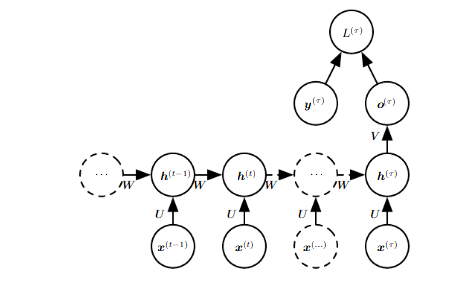
\includegraphics[width=6in]{fig/chap10/10_5.PNG} 
   \caption{这个展开的计算图只有在序列的末尾才有一个的输出。这类神经网络模型主要用来对序列进行提取抽象特征,将之表示为一个固定维度的向量(embedding)用于之后的处理。在这个模型中可能每个序列会有一个目标向量来和这个输出进行比较,也有可能使用后向传播算法的时候有梯度信息从之后的模块中流过来。}
   \label{fig:10_5}
\end{figure}

具有从输出到模型递归联系的的模型,可以通过教师驱动(teacher forcing)来训练\footnote{译者注:有的论文中也喜欢叫oracle}。教师驱动是从最大似然准则衍生出来的,在训练过程中,模型会接受到输出的真实值$y^{(t)}$作为$t+1$的输入。我们可以通过下面只有两个时间步序列的例子来了解一下这个方法。条件最大似然准则是:
\begin{align}
 &\log p(\Vy^{(1)},\Vy^{(2)} ~|~ \Vx^{(1)}, \Vx^{(2)} ) \\
 &= \log  p(\Vy^{(2)} ~|~\Vy^{(1)}, \Vx^{(1)}, \Vx^{(2)} )  + \log p(\Vy^{(1)} ~|~ \Vx^{(1)}, \Vx^{(2)}) .
\end{align}

\begin{figure}[htbp] %  figure placement: here, top, bottom, or page
   \centering
   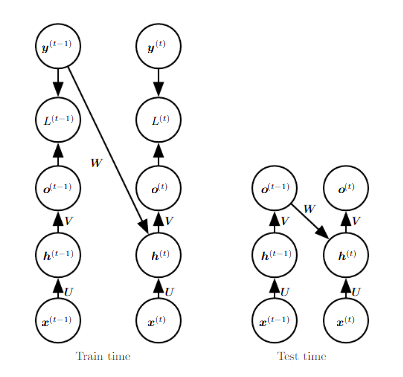
\includegraphics[width=6in]{fig/chap10/10_6.PNG} 
   \caption{ 这个图展示了教师驱动。教师驱动是一种训练技巧,常常用于输出与下一个时间点的隐藏状态有连接的循环神经网络。(左边)在训练过程中我们将$t$时刻对应的真实值$\Vy^{(t)}$ 作为输入传递给下一个隐藏节点$\Vh^{(t+1)}$。(右边)当我们真正使用这个模型或者测试的时候,真实值是不知道的,我们就会用我们模型自己做的预测值$\Vo^{(t)}$来近似代替$\Vy^{(t)}$传递给下一个隐藏状态。这里就形成了一个反馈}
   \label{fig:10_6}
\end{figure}
在这个例子中,我们看到在$t=2$的时刻,模型希望通过训练来实现在给定当前的序列$\Vx$和之前的训练集的输出$\Vy$条件下,最大化$\Vy^{(2)}$的条件概率。最大化似然是在训练过程中实现的,而不是将输出反馈给模型来实现的。我们在训练过程中不会将输出反馈给模型。我们需要传递给模型目标值,来告诉模型正确的输出是什么样的。这在图\ref{fig:10_6}做了说明。

这个模型虽然不是很强大,但是它没有隐藏到隐藏之间的联系,我们算梯度的时候就不需要像传统的RNN一样,根据时间一步一步进行后向运算。教师指导在模型拥存在隐藏节点到隐藏节点关系的时候也会被应用到模型中,只要模型当前时间点的输出与后面某个需要计算值之间存在联系我们就可以使用。但是,只要隐藏单元是历史信息的函数,我们就需要使用BPTT算法。一些模型会同时用教师指导和BPTT来进行训练。

如果之后模型会在\textbf{开环}(open-loop)模式下使用,此时网络输出(如果输出是一个概率分布或者服从某个概率分布,也有可能是输出分布样本)会被作为输入重新反馈到模型中,如果我们使用严格的教师指导来进行训练,这个时候会产生一些问题。在这种情况下,网络在训练过程中看到的输入的种类会和测试的时候看到的输入的分布会非常不一样\footnote{译者注 原文是kind,本人感觉应该是输入分布的不同,校对者来做最终的决定}。一种缓和这个问题的方式是同时使用教师指导下的输入(目标值)和模型自己产生的输出作为输入,比如说通过展开的输入到输出联系预测未来几个时间点正确的目标值。在这个方式下,网络可以学习那些没有在训练过程中见到过输入(比如说那些通过自由运转模式自己生成的输出作为的输入)以及学习如何将这个状态映射到是能够使网络在未来的几步产生合适输出。另一个方法(Bengioet al., 2015b)来解决训练过程中的输入和测试集输入不同的方式是随机选择生成的输出作为输入或者用目标值作为输入。这个方法使用了一个课程学习策略(curriculum learning strategy),它会逐渐的使用更多的生成的值来取代目标值作为输入。

\subsection{计算循环神经网络的梯度}
\label{sec:10.2.2}
计算循环神经网络的梯度是很直接的。只需要将\ref{sec:6.5.6}介绍的后向算法稍微修改一下就可以在展开图中使用,来计算梯度。通过后向算法得到的梯度随后可以被用于任何基于梯度的优化方法来训练RNN。

为了方便大家理解BPTT算法如何运作,我们提供了一个例子来展示如何通过BPTT来给RNN计算梯度(等式\ref{eq:108a}和\ref{eq:1012L})。我们计算图的节点包括参数$\MU,\MV,\MW, \Vb$和$\Vc$,以及以$t$为索引的序列节点$\Vx^{(t)}, \Vh^{(t)},\Vo^{(t)}$和$L^{(t)}$。对于每一个节点$\TSN$,我们需要递归地计算梯度$\nabla_{\TSN} L$,计算过的梯度会传递给计算图中前面的节点,在计算前面节点的梯度的时候会用到后面节点对应的梯度。递归从损失函数对应的那个节点开始:
\begin{align}
 \frac{\partial L}{\partial L^{(t)}} = 1.
\end{align}
在这个导数表达中,为了是最终的预测值$\hat{\Vy}$为归一化的概率向量,我们假定输出$\Vo^{(t)}$ 被传递给softmax函数。我们还假设损失函数为给定输入之后对目标值的负对数似然估计。对$t$时刻输出在损失函数上的梯度$\nabla_{\Vo^{(t)}} L$,它的第$i$项可以这样计算:
\begin{align}
 (\nabla_{\Vo^{(t)}} L)_i =  \frac{\partial L}{\partial o_i^{(t)}} 
 =  \frac{\partial L}{\partial L^{(t)}}  \frac{\partial L^{(t)}}{\partial o_i^{(t)}}  
 = \hat y_i^{(t)} - \mathbf{1}_{i,y^{(t)}}.
\end{align}
之后我们可以从序列的最后一项开始,逐步向前进行后向算法。最后的时间步$\tau$对应的项 $\Vh^{(\tau)}$只有$\Vo^{(\tau)}$作为后续节点,因此这个序列计算起来很简单:
\begin{align}
 \nabla_{\Vh_{(\tau)}} L = \MV^\top \nabla_{\Vo^{(\tau)}} L.
\end{align}
我们接着可以迭代地从时刻$t=\tau-1$到$t=1$进行后向计算,来随着时间后向传播梯度。$\Vh^{(t)}(t < \tau)$同时具有$\Vo^{(t)}$和$\Vh^{(t+1)}$两个后继节点。所以它的梯度用如下的方式进行计算:
\begin{align}
  \nabla_{\Vh_{(\tau)}} L = \Big( \frac{\partial \Vh^{(t+1)}}{ \Vh^{(t)}}  \Big)^\top(\nabla_{\Vh^{(t+1)}} L) 
  + \Big( \frac{\partial \Vo^{(t)}}{ \Vh^{(t)}}  \Big)^\top (\nabla_{\Vo^{(t)}} L) \\
  = \MW^\top (\nabla_{\Vh^{(t+1)}} L) \text{diag} \Big( 1 - (\Vh^{(t+1)})^2 \Big) 
  + \MV^\top \nabla_{\Vo^{(\tau)}} L,
\end{align}
其中$\text{diag} \Big( 1 - (\Vh^{(t+1)})^2 \Big) $ 表示一个包含元素$1 - (h_i^{(t+1)})^2$的对角矩阵。这是时刻$t+1$对应隐藏单元$i$(激活函数为双曲正切)对应的雅可比矩阵(Jacobian)。

一旦获得了计算图中的内部节点的梯度,我们可以获得参数节点的梯度。因为这些参数是在所有的时间节点是被共享的。在对这些参数进行求导计算的时候是要多加小心。我们需要根据\ref{sec:6.5.6}中介绍的bprop实现的方式,来计算计算图中每条边对梯度的贡献。但是,微积分中的$\nabla_{\MW} f$算子,计算$\MW$对于$f$的贡献时将计算图中\emph{所有}边都考虑进去了。为了消除这个歧义,我们引入哑变量$\MW^{(t)}$,他是$\MW$的副本,但是只在$t$时刻使用。我们可能用$\nabla_{\MW^{(t)}}$来表示,$t$时刻对应的权重对梯度的贡献。

通过这些符号,其他参数的梯度可以这样计算:
\begin{align}
 \nabla_{\Vc} L &=  \sum_t \Big( \frac{\partial \Vo^{(t)}}{\partial \Vc} \Big)^\top \nabla_{\Vo^{(t)}} L 
 = \sum_t \nabla_{\Vo^{(t)}} L ,\\
 \nabla_{\Vb} L &= \sum_t \Big( \frac{\partial \Vh^{(t)}}{\partial \Vb^{(t)}} \Big)^\top \nabla_{\Vh^{(t)}} L 
 = \sum_t \text{diag} \Big( 1 - \big( \Vh^{(t)} \big)^2 \Big)  \nabla_{\Vh^{(t)}} L  ,\\
 \nabla_{\MV} L &= \sum_t \sum_i \Big( \frac{\partial L} {\partial o_i^{(t)}}\Big) \nabla_{\MV} o_i^{(t)} 
 = \sum_t (\nabla_{\Vo^{(t)}} L) \Vh^{(t)^\top},\\
 \nabla_{\MW} L &= \sum_t \sum_i \Big( \frac{\partial L} {\partial h_i^{(t)}}\Big) 
 \nabla_{\MW^{(t)}} h_i^{(t)} \\
&= \sum_t \text{diag} \Big( 1 - \big( \Vh^{(t)} \big)^2 \Big) ( \nabla_{\Vh^{(t)}} L) \Vh^{(t-1)^\top} ,\\
 \nabla_{\MU} L &= \sum_t \sum_i \Big( \frac{\partial L} {\partial h_i^{(t)}}\Big) 
 \nabla_{\MU^{(t)}} h_i^{(t)} \\
&= \sum_t \text{diag} \Big( 1 - \big( \Vh^{(t)} \big)^2 \Big) ( \nabla_{\Vh^{(t)}} L) \Vx^{(t)^\top} 
\end{align}

我们不需要在训练的时候计算损失函数对输入$\Vx^{(t)}$的梯度,因为梯度是用于更新参数的,而输入节点的后面没有参数节点了,所以没有必要计算他们对应的梯度。

\subsection{把循环神经网络看作有向图模型}
我们目前介绍的循环神经网络的例子中,损失函数$L^{(t)}$是训练目标$\Vy^{(t)}$和输出$\Vo^{(t)}$之间的交叉熵。循环神经网络也是前馈网络的一种,所以我们其实可以使用任意的的损失函数。我们需要根据任务来寻找合适的损失函数。作为一个前馈网络,我们通常希望RNN的输出可以被看作是概率分布,随后我们可以根据输出分布来与目标之间的交叉熵来定义损失。举个例子,前馈神经网络中,如果输出是高斯单元的话,均方误差就是交叉熵损失。

但我们使用一个预测目标时的对数似然训练过程中的目标函数,比如说等式\ref{eq:1012L},我们在训练RNN的时候,在给定前面的序列元素的条件之下,估计下一个序列元素的条件分布。这个可以看作最大化对数似然
\begin{align}
 \log p(\Vy^{(t)} \mid \Vx^{(1)},\dots, \Vx^{(t)}),
\end{align}
或者,如果模型包含从某一结点输出到下一节点的联系时,
\begin{align}
 \log p(\Vy^{(t)} \mid \Vx^{(1)},\dots, \Vx^{(t)},\Vy^{(1)},\dots, \Vy^{(t-1)} ).
\end{align}
把整个输出序列$\Vy$的联合概率分解为基于一系列单步的概率预测相乘的形式,可以帮助我们获得整个序列的联合概率分布。当我们不再把$\Vy$值作为预测下一个元素的条件时,这个有向图模型不再包含任何从过去$\Vy^{(i)}$到当前$\Vy^{(t)}$的边。在这个情况下,当给定序列$\Vx$的值的作为条件的时候,输出$\Vy$里面的元素是条件独立的。但我们反馈给网络当前真实的$\Vy$值(不是对应的预测值,而是真正观测到或生成的值),那么有向图模型包含了所有的从过去$\Vy^{(i)}$到当前$\Vy^{(t)}$的边。

举一个简单的例子,我们想象一个RNN模型只处理一个标量随机变量序列$ \SetY = \{\RSy^{(1)},\dots,\RSy^{(\tau)}\}$,没有额外的输入$\RSx$。里面的每个值是随机变量,没有其他额外的输出x。$t$时刻的输入时$t-1$时刻的输出。RNN为这$\RSy$个变量定义了一个有向图模型。我们使用链式法来利用条件概率参数化这些观测值的联合分布:
\begin{align}
 P(\SetY) = P(\RVy^{(1)},\dots,\RVy^{(\tau)}) = \prod_{t=1}^{\tau}P(\RVy^{(t)} \mid \RVy^{(t-1)},\RVy^{(t-2)},
 \dots,\RVy^{(1)}),
\end{align}
当$t=1$时,竖杠右侧显然为空。因此,根据这样一个模型,这一系列值$\{y^{(1)},\dots,y^{(\tau)} \}$的负对数似然为
\begin{align}
 L = \sum_{t} L^{(t)},
\end{align}
其中, 
\begin{align}
 L^{(t)} = -\log P(\RSy^{(t)} = y^{(t)} \mid y^{(t-1)},y^{(t-2)}, \dots, y^{(1)}).
\end{align}

\begin{figure}[htbp] %  figure placement: here, top, bottom, or page
   \centering
   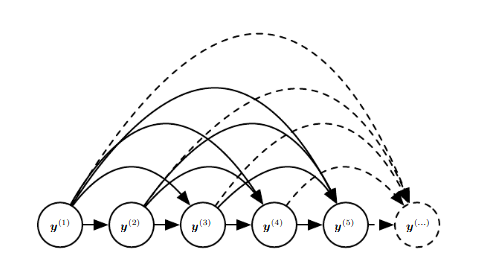
\includegraphics[width=6in]{fig/chap10/10_7.PNG} 
   \caption{ 序列$\RSy^{(1)},\RSy^{(2)},\dots,\RSy^{(t)},\dots$对应的全连接的图模型。之前的观测值$\RSy^{(i)}$,会影响未来的观察值$\RSy^{(t)}(t>i)$的条件分布。直接参数化这个图模型会有点麻烦,因为随着输入的增加参数也会大量增加。RNN也是一个全连接结构,但是它使用了较少的参数,可以看一下图\ref{fig:10_8}来进行一下对比。}
   \label{fig:10_7}
\end{figure}

\begin{figure}[htbp] %  figure placement: here, top, bottom, or page
   \centering
   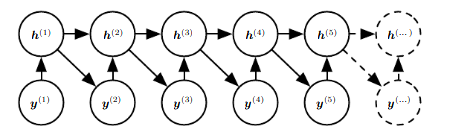
\includegraphics[width=6in]{fig/chap10/10_8.PNG} 
   \caption{ 展示了RNN代表的图模型的状态变量,尽管输入到状态变量的映射是一个固定的函数,但是它可以帮助我们使用较少的参数来参数化\ref{form:10.5}我们的模型。序列中的每一个步骤都使用了相同的结构(每个节点具有相同的输入维度),并且这些结构每一步共享它们的参数。}
   \label{fig:10_8}
\end{figure}

图模型中的边表示的是变量之间的依赖关系。很多图模型期望可以通过省略一些没有很强交互性的边来换取统计和计算的效率。举个例子,通常我们会假设图模型具有马尔科夫性。这个时候图中只包含从$\{ \RSy^{(t-k)}, \dots, \RSy^{(t-1)}\}$到$\RSy^{(t)}$的边,而不是包含所有从历史节点到当前结点的边。但是在有的情况下,我们相信所有的历史的输入对序列的下一个元素都有影响。当我们认为$\RSy^{(t)}$的分布可能取决于过去的某个节点$y^{(i)}$,且无法通过$y^{(t-1)}$获得$y^{(i)}$的信息时,RNN就可以大显身手。

当我们用图模型的解释RNN的时候,我们可以把RNN看作是一个全连接的图模型。这是表示任何一对的$y$之间都有依赖关系。图\ref{fig:10_8}是$y$值之间具有全连接结构的图模型。
我们在学习这个RNN代表的完全图的时候通过边缘化\footnote{译者注:概率统计有介绍,把某个随机变量的所有值累加起来}的方式消去了模型中的隐藏单元$\Vh^{(t)}$。

当我们把RNN看作是一个图模型的时候,我们可以把隐藏单元$\Vh^{(t)}$看作是随机变量\footnote{给变量的父节点之后,那些变量的条件分布就确定了。
尽管设计具有这样隐藏单元具有确定分布的图模型是很少见的,但这是完全合理的。}。
在RNN对应的图模型中包括隐藏单元,说明我们可以非常有效的参数化观测的联合分布。
假设我们用表格(tabular representation)来表示某些离散变量上任意的联合分布,在表格中,任意的离散变量的组合都对应着一个小格子,里面的值代表这个组合发生的概率。
如果$y$可以取$k$个不同的值,表格将会有$\CalO(k^\tau)$个参数。
但是RNN由于参数共享,它的参数数目为$\CalO(1)$,是序列长度的函数\footnote{译者注:此处存疑,感觉是作者笔误,复杂度应该为常数}
我们可以调节参数数量来控制RNN的模型容量,但参数数目不会随着序列长度增加而增加。
等式\ref{eq:105h}展示了RNN通过递归掉用相同的函数$f$以及在每个时间点的使用相同参数$\Vtheta$,有效地参数化的变量之间的联系,即使这些变量之间的距离可能很长。
可以通过图\ref{fig:10_8}加深我们对RNN所代表的图模型的理解。
在图模型中,如果我们给定$\Vh^{(t)}$节点,这个节点是过去和未来的中间节点,这个时候,过去和未来就相互独立了。
过去的某个变量$y^{(i)}$可以通过$\Vh$来影响未来的某个变量$y^{(t)}$。
在这个图模型中,我们对每个时间步都使用相同的条件概率分布,这样就可以高效地参数化模型,并且当观察到全部变量时,可以高效地评估联合分布分配给所有变量的概率\footnote{译者注:此处不是很清晰}。

虽然我们可以高效地参数化图模型,某些操作在计算上依然具有挑战性。
比如说,难以预测在序列中间缺少的值。

虽然循环神经网络的参数数目并不多,但是参数\emph{优化}可能会变困难。

我们之所以在循环神经网络中使用的参数共享,是因为我们假设相同参数可用于序列不同的位置。
同样的,这个也是假设在给定时刻$t$的变量的条件下,在时刻$t +1$变量的条件概率分布是固定的stationary,这意味着序列不同位置的变量之间的关系并不依赖于位置$t$。
原则上,可以使用$t$作为每个时间步的额外输入,并让学习器在发现任何时间依赖性的同时,在不同的时间步之间尽可能多地共享这个信息。
相比在每个位置$t$使用不同的条件概率分布,这个策略已经好很多了,但网络将必须在面对新$t$时进行推断更新。

为了更全面的吧RNN用图模型来解释,我们必须描述如何从这个模型中进行采样。
我们要做是每个不同的时间步的条件分布中进行采样。
然而,这儿有一个小麻烦。RNN必须有某种机制来确定序列的长度。当然,这可以通过很多方式来实现。

在当输出是属于某个词汇表中的符号时,我们可以在词汇表中添加一个特殊符号来表示序列终止(Schmidhuber, 2012)。
当这个符号出现时,采样过程停止。
在训练集中,我们将该符号作为一个额外成员插入序列的末尾,即紧跟每个训练样本$\Vx^{(\tau)}$之后。

另一种方法是在模型中引入一个额外的Bernoulli输出,表示在每个时间步之后决定继续生成还是终止。
这种方法比向词汇表增加一个额外符号的方法使用的更广泛,因为它可以适用于任何RNN模型,而不仅仅用于输出符号序列的RNN模型。
例如,它可以应用于一个产生实数序列的RNN模型。
新的输出单元通常使用sigmoid单元,损失函数则为交叉熵。
在这种方法中,sigmoid被训练为最大化正确预测的对数概率,即在每个时间步决定序列是否结束\footnote{译者注:此处不是很懂}。

确定序列长度$\tau$的另一种方法是将一个额外的输出添加到模型用来预测$\tau$本身。
模型可以采样出一个$\tau$的值,然后采样$\tau$步有价值的数据。
这种方法需要在每个时间步的循环更新的时候增加一个额外输入,使得循环在更新的时候知道它是否是靠近所产生序列的末尾\footnote{译者注:更新应该指的是产生条件概率}。
这种额外的输入可以是$\tau$的值,也可以是$\tau - t$,即剩下时间步的数量。
如果没有这个额外的输入,RNN可能会突然结束序列的产生,例如在产生句子时,可能句子还没有完整,生成就结束了。
这个方法可以用下面这个式子来解释:
\begin{align}
 P(\Vx^{(1)},\dots, \Vx^{(\tau)}) = P(\tau) P(\Vx^{(1)},\dots,\Vx^{(\tau)} \mid \tau) .
\end{align}
直接预测$\tau$的例子请参考 Goodfellow et al.(2014d)。

\subsection{通过RNN基于上下文对序列进行建模}
在上一小节,我们描述了如何从概率图模型的角度来看待RNN,还举了一个例子,在这个例子里没有输入$\Vx$,直接对随机变量序列$y^{(t)}$进行建模。当然,传统的RNN如等式\ref{eq:108a}所示,包含一个输入序列$\Vx^{(1)},\Vx^{(2)},\dots,\Vx^{(\tau)}$。一般情况下,我们在用图模型解释RNN的时候,不仅可以表示$y$变量的联合分布也能表示给定$\Vx$条件下,$y$条件分布。正如我们在\ref{sec:6.2.1.1}中介绍的前向网络一样,任何可以表示为$P(\Vy;\Vtheta)$的模型都能被重新写成条件分布$P(\Vy \mid \Vomega)$的形式,其中$\Vomega=\Vtheta$。
同样的,我们可以通过使用$P(\Vy \mid \Vomega)$代表分布$P(\Vy \mid \Vx)$来扩展这样的模型,但要令$\Vomega$是关于$\Vx$的函数。在RNN中,这个条件可以用多种不同的方式来实现。此处我们回顾一下最常用最有效的一些方法。

之前,我们已经讨论了将的向量$\Vx^{(t)}$序列作为输入传递给RNN,其中$t =1, \dots, \tau$。RNN也可以接受单个向量$\Vx$作为输入。
当$\Vx$是一个固定大小的向量,我们可以简单地将其看作产生$\Vy$序列RNN的一个额外输入。
将额外输入传递给RNN的一些常见方法是:
\begin{enumerate}
 \item 在每个时刻作为一个额外输入,或
 \item 把$\Vx$作为初始状态$\Vh^{(0)}$,或
 \item 两种方式同时使用。
\end{enumerate}

第一个也是最常用的方法在图\ref{fig:10_9}中进行了说明。
输入$\Vx$和每个隐藏单元向量$\Vh^{(t)}$之间的联系通过新引入的权重矩阵$\MR$来进行参数化的,这个权重矩阵在只包含$y$序列的模型中是没有的。
同样的,$\Vx^\top\MR$在每个时间步会作为隐藏单元的一个额外输入。
我们可以认为在确定$\Vx^\top\MR$值的时候,$\Vx$的选择可以看作是每个隐藏单元的一个偏置参数。
权重与输入保持独立。
我们可以把这种模型看作是由参数$\Vtheta$决定的非条件模型,我们可以把$\Vtheta$改成$\Vomega$,这时$\Vomega$里面的偏置参数是输入的函数。
\begin{figure}[htbp] %  figure placement: here, top, bottom, or page
   \centering
   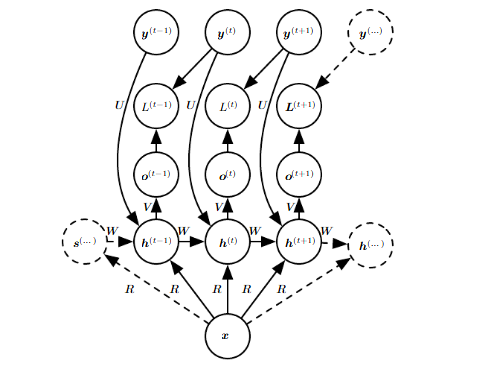
\includegraphics[width=6in]{fig/chap10/10_9.PNG} 
   \caption{ 在这个图中,RNN将一个固定长度的向量$\Vx$映射为一个序列$Y$的分布。在做图像说明(image captioning)任务的时候我们常常使用这类模型。此时,图像就作为模型的输入,模型需要输出一个单词序列来描述这个图片。每个已观察到的输出序列里的元素$\Vy^{(t)}$会作为输入(给当前的时间步),同时它也是目标值(针对的是之前时间步)。}
   \label{fig:10_9}
\end{figure}

除了接收单个的一个向量作为输入以外,RNN也可以接收向量序列$\Vx^{(t)}$作为输入。等式\ref{eq:108a}描述的RNN对应的条件分布是$P(\Vy^{(1)}, \dots, \Vy^{(\tau)} ~|~ \Vx^{(1)}, \dots, \Vx^{(\tau)})$,根据条件独立性假设\footnote{译者注:在给定历史的输入$\Vy^{(t)} \mid \Vx^{(1)}, \dots, \Vx^{(t)}$的条件之后,$\Vy^{(t)}$直接相互条件独立}这个分布可以分解为
\begin{align}
 \prod_t P(\Vy^{(t)} \mid \Vx^{(1)}, \dots, \Vx^{(t)}).
\end{align}
为消除条件独立的假设,我们可以给在时刻$t$的输出到时间$t+1$的隐藏单元之间添加连接,如图\ref{fig:10_10}所示。
该模型就可以表示$\Vy$序列的任意概率分布。
这种给定一个序列的条件下表示另一个序列分布的模型的还是有一个限制,就是这给定序列和要表示的序列长度必须相等。在\ref{sec:10.4}我们介绍了如何取消这个限制条件。
\begin{figure}[htbp] %  figure placement: here, top, bottom, or page
   \centering
   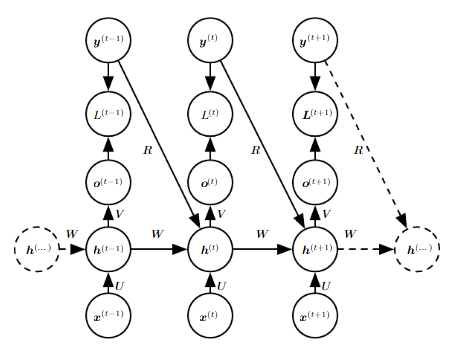
\includegraphics[width=6in]{fig/chap10/10_10.PNG} 
   \caption{ 这是一个条件循环神经网络(conditional recurrent neural network),长度不定的输入序列$\Vx$映射成为一个和输入具有相同长度的序列$\Vy$的分布。和图\ref{fig:10_3}相比,这个模型中多了输出到下一状态节点之间的联系。这些联系可以帮助RNN给定序列$\Vx$的条件下,对$\Vy$的任意分布进行建模。而图\ref{fig:10_3}对应的模型在对$\Vy$进行建模时,必须保证给定$\Vx$的条件下,$\Vy$条件独立。}
   \label{fig:10_10}
\end{figure}
\section{双向RNN(Bidirectional RNNs)}
\label{sec:10.3}
目前为止我们考虑的所有RNN模型的例子都是“因果”结构的,意味着在时刻$t$的状态只能从历史序列$\Vx^{(1)},\dots,\Vx^{(t-1)}$以及当前的输入$\Vx^{(t)}$中获得信息。
在一些例子中,我们还讨论了在训练过程中,使用过去的目标值$\Vy$来影响当前状态。

但是,在许多应用中,我们要输出的预测$\Vy^{(t)}$可能依赖于整个输入序列。举个例子,在语音识别中,由于协同发音(co-articulation),语音会被分解成音素(phoneme),当前的语音所对应的音素的可能取决于未来几个音素,甚至由于相邻的单词之间存在语义依赖,该音素可能取决于未来的几个单词:如果当前的词有两种声学上合理的解释,我们可能要在更远的未来(和过去)来寻找信息从两个中选择一个正确的。
这在手写识别和许多其他序列到序列的学习任务中也是如此,将会在下一节对这类问题进行描述。

发明双向递归神经网络(bidirectional RNNs)的发明就是为了解决上一段提到的那些问题(Schuster and Paliwal, 1997)。当需要处理的任务有这种需求时,双向循环神经网络获得了非常大的成功 (Graves, 2012),比如说手写识别 (Graves et al., 2008; Graves and Schmidhuber, 2009), 语音识别 (Graves and Schmidhuber, 2005; Graves et al., 2013) 以及生物信息学 (Baldiet al., 1999)。

顾名思义,双向循环神经网络由两个循环神经网络组成,一个是前向(forward)循环神经网络:从序列的开始向后处理数据。另一个事后向(backward)循环神经网络:从序列的的末尾向前处理数据。
图\ref{fig:10_11}展示了典型的双向循环神经网络的结构,其中$\Vh^{(t)}$是前向循环神经网络的状态节点,$\Vg^{(t)}$是后向循环神经网络的状态节点。
这时输出单元$\Vo^{(t)}$就可以同时考虑过去和未来的信息。当然$\Vo^{(t)}$的值对时刻$t$的输入值是很敏感的。此时我们不必像前馈神经网络,卷积神经网络或者是一个单向的具有固定大小的先行缓存器( look-ahead buffer)的RNN一样,在$t$周围指定一个固定大小的窗口。模型可以获得这个窗口里面输入的信息。

\begin{figure}[htbp] %  figure placement: here, top, bottom, or page
   \centering
   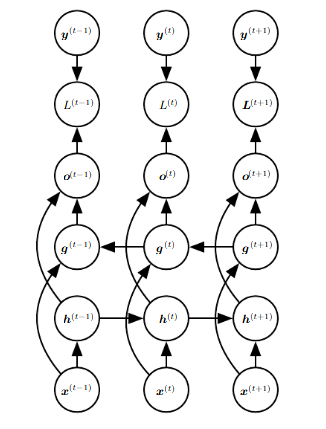
\includegraphics[width=6in]{fig/chap10/10_11.PNG} 
   \caption{一个典型的双向循环神经网络计算图,学习任务是将输入序列$\Vx$映射到目标序列$\Vy$,每一步的损失为$L^{(t)}$,$\Vh$的信息循环向前传播(从左往右),$\Vg$的信息循环向后传播(从右往左)。所以$\Vh^{(t)}$中包含了过去的输入信息而$\Vg^{(t)}$中包含了未来的输入信息,输出单元$\Vo^{(t)}$会同时参考$\Vh^{(t)}$和$\Vg^{(t)}$,那么也就可以同时考虑过去和未来的输入信息}
   \label{fig:10_11}
\end{figure}

这个想法可以扩展到2维的输入数据,比如说图像,这时我们就需要\emph{四个}RNN,沿着四个方向(上、下、左、右)来对数据进行处理。
如果循环神经网络能够学习到更多的上下文信息,那在计算2维网格上的每个点$(i, j)$的输出$O_{i,j}$就能可以不仅仅只考虑局部信息,还能够考虑距离位置$(i, j)$更远的信息。
相比于卷积神经网络,在图像上使用RNN通常更复杂,但RNN就允许特征图的特征之间存在长期横向的相互作用\footnote{译者注:卷积神经网络只可以考虑到局部的联系,即只能考虑到那个固定窗口里面的信息,而循环神经网络则可以获得更广的上下文信息,不过四向RNN应用的很少}(Visin et al., 2015; Kalchbrenner et al., 2015)。
实际上,对于这样的循环神经网络模型,前向传播公式可以写成卷积的形式,在包含横向联系的特征图上进行递归计算之前,在每一层自底向上对输入进行处理\footnote{译者注:原文表达不清晰,不知道怎么翻译}。

\section{基于编码-解码的序列到序列架构}
\label{sec:10.4}
我们已经在图\ref{fig:10_5}看到RNN如何将输入序列映射成固定大小的向量,在图\ref{fig:10_9}中展示了RNN如何将固定大小的向量映射成为一个序列,在图\ref{fig:10_3}、\ref{fig:10_4}、\ref{fig:10_10}和\ref{fig:10_11}中看到RNN如何将一个输入序列映射到与输入等长的输出序列。

本节我们讨论如何训练RNN,使其将输入序列映射到任意长度的输出序列。
这在许多机器学习任务中都有使用,如语音识别、机器翻译或问答系统,其中训练集的输入和输出序列的长度通常不相同(虽然它们的长度可能有联系)。

\begin{figure}[htbp] %  figure placement: here, top, bottom, or page
   \centering
   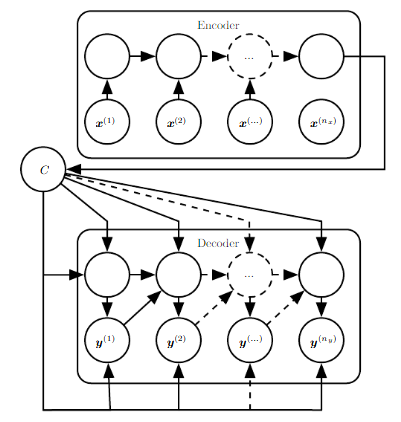
\includegraphics[width=4in]{fig/chap10/10_12.PNG} 
   \caption{基于编码-解码的序列到序列架构的一个实例。根据输入序列$(\Vx^{(1)},\Vx^{(2)} \dots, \Vx^{(n_x)})$产生输出序列$(\Vy^{(1)},\Vy^{(2)} \dots, \Vy^{(n_y)})$。这个模型有两部分RNN组成,第一个编码RNN用来读入序列,第二个解码RNN用来产生输出序列(或者说计算输出序列的分布)。编码RNN的最后一个隐藏状态可以用固定大小的变量$C$(contex)来表示,$C$里面存储这对输入序列语义的总结信息。$C$也会作为输入传递给解码RNN用来生成输出序列。}
   \label{fig:10_12}
\end{figure}

我们通常较RNN的输入为\textbf{上下文}(contex),我们通常用$C$来表示上下文信息。
这个上下文$C$可能是对输入序列$\MX=(\Vx^{(1)},\dots,\Vx^{(n_x)})$信息的概括。他可以是向量或者向量序列。

用于将长度不定的序列映射到另一一个长度不定序列的RNN架构最初由 Cho et al. (2014a)提出,不久之后 Sutskever et al. (2014)对这个架构进行了发展,并把这种方法应用到机器翻译翻译中,取得了较好结果。这个系统是对另一个机器翻译系统产生的翻译结果进行评分,而后者使用一个传统的递归神经网络来生成翻译结果。
这些作者对这个架构\ref{fig:10_12}不同的称呼,通常叫编码-解码或序列到序列架构。
这个架构的本质非常简单:(1)用\textbf{编码}或\textbf{读取器}(reader)或\textbf{输入}(input)RNN接收输入序列。
这个编码RNN最后会输出上下文$C$(通常是对最后一个隐藏状态进行处理输出)。
(2)\textbf{解码}或\textbf{写入器}(writer)或\textbf{输出}(output)RNN则接收固定长度的向量$C$(如图\ref{fig:10_9})然后生成输出序列$\MY=(\Vy^{(1)}, \dots, \Vy^{(n_y)})$。
这种架构的创新之处在于输入输出序列的长度$n_x$和$n_y$可以彼此不同,而前面介绍的RNN的架构基本都要求输入序列长度等于输出序列长度$n_x = n_y = \tau$。
在这个序列到序列的架构中,我们需要同时训练这两个RNN来最大化训练集中所有$\Vx$和$\Vy$对数条件概率$\log P( \Vy^{(1)}, \dots, \Vy^{(n_y)} ~|~ \Vx^{(1)},\dots,\Vx^{(n_x)} )$。
编码RNN的最后一个隐藏状态$\Vh_{n_x}$通常被当作输入的上下文$C$,或者是输入序列信息的总结,并作为解码RNN的输入。

如果上下文$C$是一个向量,则解码RNN的结构和我们在\ref{sec:10.2.4}节介绍的一样,是一个将向量映射到序列RNN结构。
正如之前介绍的那样,将向量映射到序列的RNN至少有两种方式来接受输入向量。
输入可以作为RNN的初始状态,或也可以作为输入传给每一个时间步中隐藏单元。这两种方式也可以结合起来使用。

这个结构并不限制编码RNN和解码RNN具有相同大小的隐藏层。

但是这个架构有一个明显的不足:如果编码RNN输出的上下文$C$的维度太小,它不能将输入序列的有用的信息全部存进这个向量$C$。
这是由 Bahdanau et al. (2015)在用这个架构做机器翻译的时候观察到的。
他们提出让$C$成为长度可变的序列,而不是一个固定大小的向量。
此外,他们还介绍了注意力机制(attention mechanism),将序列$C$的元素和输出序列的元素相关联起来。更多的细节会在\ref{sec:12.4.5.1}进行介绍。

\section{深度RNN结构}
\label{sec:10.5}
大多数RNN的计算可以分为三个模块,当然也对应着三组参数和三个变换映射:
\begin{enumerate}
 \item 从输入到隐藏状态,
 \item 从前一隐藏状态到下一隐藏状态,
 \item 从隐藏状态到输出。
\end{enumerate}
\ref{fig:10_3}是传统的RNN的结构,这三个模块每个都有一个与之相关的权重矩阵。或者说,当我们把RNN展开时,每个模块对应一个简单的变换,而这个变化是可以用单层或者多层的MLP来表示的。通常这个转换分为两步,显示一个仿射变换,紧接着把仿射变换的结果进行非线性变换\footnote{sigmoid,tanh}。

那么如果我们使用更复杂的变换,或者原来只有一层的MLP,我们把它变成多层,这样会不会让我们的模型有一个更好的表现呢?
 (Graves et al., 2013; Pascanu et al., 2014a)里的实验证明了这一点。我们需要足够深的网络结构来获得理想的变换映射。 一些早期深度RNN的介绍可以参考 Schmidhuber (1992),El Hihi and Bengio (1996), 或者 Jaeger (2007a)。
 
 Graves et al.(2013) 首先发现了像\ref{fig:10_13}(左)一样,将RNN的状态分为多层可以给模型的表现带来显著的提升,如。
我们可以认为,在\ref{fig:10_13}(a)所示在多层结构中最开始的那些层主要将原始输入进行抽象转换,输出一个对隐藏状态更合适,更高层次的表示。
Pascanu et al. (2014a)进一步提出在上述三个模块中分布使用一个单独的MLP结构(可以是多层的),如\ref{fig:10_13}(b)所示。
考虑到模型的表示能力,我们建议在这三个模块合理分配足够的容量,但当我们增加模型的深度可能会造成优化困难而损害学习效果。
在一般情况下,浅层的架构更容易优化,如果我们像\ref{fig:10_13}(b)加入额外的层会导致从时间点$t$的变量到时间点$t+1$的最短路径变长。
例如,如果单隐藏层的MLP被用于状态到状态的转换,那么我们在\ref{fig:10_13}使用的结构任何两个不同时间点变量之间最短路径的长度会加倍。
然而Pascanu et al(2014a)认为,在隐藏状态到隐藏状态的路径中引入跨越连接(skip connection)如\ref{fig:10_13}(c)所示,可以缓和这个问题。

 \begin{figure}[htbp] %  figure placement: here, top, bottom, or page
   \centering
   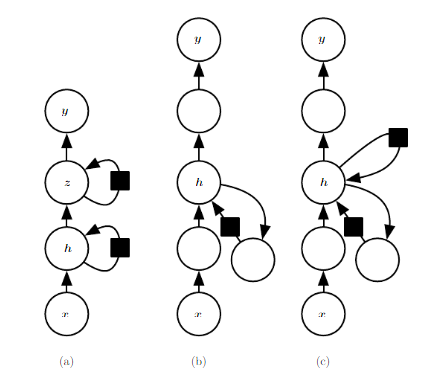
\includegraphics[width=4in]{fig/chap10/10_13.PNG} 
   \caption{一个循环神经网络可以通过不同的方式来加深网络的层数(Pascanu et al, 2014a)。(a)RNN中的隐藏状态可以被分成多组层次结构。(b)在输入到隐藏状态,隐藏到隐藏状态和隐藏到输入状态中加深结构(比如说吧MLP由一层转为多层)。这会延迟不同时间步节点之间的最短路径的长度。(c)路径延长的副作用可以通过跨越连接来缓和。}
   \label{fig:10_13}
\end{figure}

